\documentclass{article}

\usepackage[utf8]{inputenc}
\usepackage{graphicx} % Required for the inclusion of images
\usepackage{amsmath} % Required for some math elements 
\usepackage[utf8]{inputenc}
\usepackage[english]{babel}
\newtheorem{theorem}{Theorem}
\newtheorem{corollary}{Corollary}[theorem]
\newtheorem{lemma}[theorem]{Lemma}

%TODO follow the instructions on http://workspace.nottingham.ac.uk/display/CompSci/Procedure+for+PhD+Annual+Reviews

% A written report that contains the following sections. There is no specific requirement on formatting but it should be well-presented and proof-read to ensure it is a piece of high-quality academic writing. As guidance, the whole report including the appendix should normally be around 8000-10000 words in length.

%TODO Current title of PhD project, Whether it is a first, second or third annual review report, word count, student name, student ID, names of supervisors, initial registration date, expected date for entering thesis pending stage, expected date for thesis submission.
\title{1st Year Report \\ Pure Functional Methods in \\ Agent-Based Modelling \& Simulation} % Title

\author{Jonathan \textsc{Thaler} \\ jonathan.thaler@nottingham.ac.uk} % Author name

\date{\today} % Date for the report

\begin{document}
\maketitle % Insert the title, author and date

% If you wish to include an abstract, uncomment the lines below
\begin{abstract}
A succinct and concise summary (250 words maximum) of the report contents and presented on a single page.

So far specifying Agent-Based Models and implementing them as an Agent-Based Simulation (ABS) is done using object-oriented methods like UML and object-oriented programming languages like Java. The reason for this is that until now the concept of an agent was always understood to be very close to, if not equals to - which it is not - the concept of an object. Therefore, the reasoning goes, object-oriented methods and languages should fit themselves naturally to specify and implement agent-based simulations. In this PhD Thesis we fundamentally challenge this assumption by investigating how Agent-Based Models and Simulations can be specified and implemented using pure functional methods and programming in Haskell and what the benefits are. We will show that the implicit assumption that an Agent is \textit{about equal to} an Object is not correct and leads to many implicit assumptions in object-oriented implementations of Agent-Based Simulation (ABS). When implementing ABS in Haskell these implicit assumptions become explicit and challenge the fundamental assumptions about ABS and Agents. We present these implicit assumption in an explicit way by approaching it through programming, type-theory and category-theory to further deepen the concepts and methods in the field of Agent-Based Modelling \& Simulation. We also think that the major benefit of implementing ABS in Haskell is the potential for an unprecedented approach of formal validation \& verification of an Agent-Based Model and its implementation. Due to the declarative nature of pure functional programming in Haskell it is possible to implement an EDSL for ABS which ideally results in code which looks like specification thus closing the gap between specification and implementation because the specification is already the code. For validation we want to pursue testing through QuickCheck.

In this report I discuss the research conducted to far, present the open problems together with an in-depth literature review. An outline for the research of the following 2 years is given and the aims.
\end{abstract}

%TODO Contents Page Main headings with page numbers.

\section{Introduction}
There exists a large number of simulation packages which allow the convenient creation of System Dynamics simulations by straight-forward visual diagram creation. One simply creates stocks and flows, connects them, specifies the flow-rates and initial parameters and then runs the model. An example for such a visual diagram creation in the simulation package AnyLogic can be seen in Figure \ref{fig:sir_stockflow_diagram}.

\begin{figure}
	\centering
	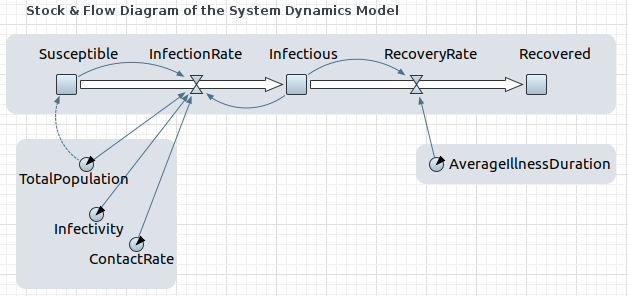
\includegraphics[width=.5\textwidth, angle=0]{./fig/SIR_SD_STOCKFLOW_DIAGRAMM.png}
	\caption{Visual System Dynamics Diagram of the SIR model in AnyLogic Personal Learning Edition 8.3.1.}
	\label{fig:sir_stockflow_diagram}
\end{figure}

Still, implementing System Dynamics directly in code is not as straight forward and involves numerical integration which can be quite tricky to get right. Thus, the aim of this paper is to look into how System Dynamics models can be implemented in code correctly without the use of a simulation package. We use the well known SIR model \cite{kermack_contribution_1927} from epidemiology to demonstrate our approach.

Our language of choice is Haskell because it emphasises a declarative programming style in which one describes \textit{what} instead of \textit{how} to compute. Further it allows to rule out interference with non-deterministic influences or side-effects already at compile-time. This is of fundamental importance for System Dynamics because it behaves completely deterministic and involves no stochastics or non-determinism whatsoever. Also, we make use of Functional Reactive Programming which allows to express continuous-time systems in a functional way. 

We show that by this approach we can arrive at correct-by-construction implementations of System Dynamic models. This means that the correctness of the code is obvious because we have closed the gap between the model specification and its implementation. Thus, the contribution of the paper is the demonstration of how to implement correct-by-construction System Dynamics simulations using Haskell and Functional Reactive Programming.

\section{Conducted Research}
TODO: Describe the research work carried out during this stage of the PhD and the outcomes. A literature review must be included. Then, as appropriate according to the PhD project, this section can also include theoretical and/or experimental methods, presentation and discussion of results, etc. In the case that papers have been submitted or published within the year of the review, this section can be shorter and focused on discussing the outcomes from those papers within the wider context of the PhD programme of study (papers to be included in the appendix).

Literature Review
- ask other students: Tuong, Olusola, Ivan for their 1st year reviews
- trichter: mit den 3 themen beginnen und dann runterbrechen und ins detail gehen, bis der gap gefunden wurde

ADOM: Agent Domain of Monads: https://www.haskell.org/communities/11-2006/html/report.html

\chapter{Conclusions}
\label{chap:concl}

\section{Being Realistic}
It is of most importance to stress that we don't condemn the current state-of-the-art approach of object-oriented specification and implementation to ABS. The strength of object-oriented programming is surely that it can be seen as \textit{programming as modelling} and thus will be always an attractive approach to ABS. Also we are realists and know that there are more points to consider when selecting a set of methods for developing software for an ABS than robustness, verification and validation. Almost always the popularity of an existing language and which languages the implementer knows is the driving force behind which methods and languages to choose. This means that ABS will continue to be implemented in object-oriented programming languages and many perfectly well functioning models will be created by it in the future. Although they all suffer from the same issues mentioned in the introduction this doesn't matter as they are not of central importance to most of them.
Nonetheless we think our work is still essential and necessary as it may start a slow paradigm-shift and opens up the minds of the ABS community to a more functional and formal way of approaching and implementing agent-based models and simulations and recognizing the benefits one gets automatically from it by doing so.

\section{What we are not doing}
Because of this highly interdisciplinary topic we explicitly mention what we do not want to undertake in this PhD.
First we don't want to develop another language for formal agent-specification which needs to be compiled or used in some fancy tool - we want to put it directly into Haskell, building on the existing facilities.
Second, we are not developing a new economic theory about decentralized bilateral bartering, we take the existing theory and existing agent-based models and apply our methods to them.
Third, we don't want to use fancy statistics and number juggling for comparing validating and verifying models: we want structural comparison (category-theory).
Fourth, we do NOT want to do a direct comparison of object-orientation vs. functional in ABS, as we would get lost in an infinite amount of low-level technical details. We look at the benefits / drawbacks more on a conceptual level, applied to ABS.

\section{Future Work Plan}
TODO: A future work plan that is consistent with the progress to date, stating clearly the research question(s) to be addressed during the next year of the PhD.

%\bibliographystyle{acm}
\bibliography{../../references/phdReferences}

\begin{appendices}

\chapter{Pure Functional Epidemics}
\label{app:pfe}
Submission history:
\begin{enumerate}
	\item Submitted to Haskell Symposium 2018 on 30th March \\ REJECTED on 18th May
	\item Submitted to IFL 2018 on 25th May \\ NOTIFICATION PENDING until 20th July
\end{enumerate}

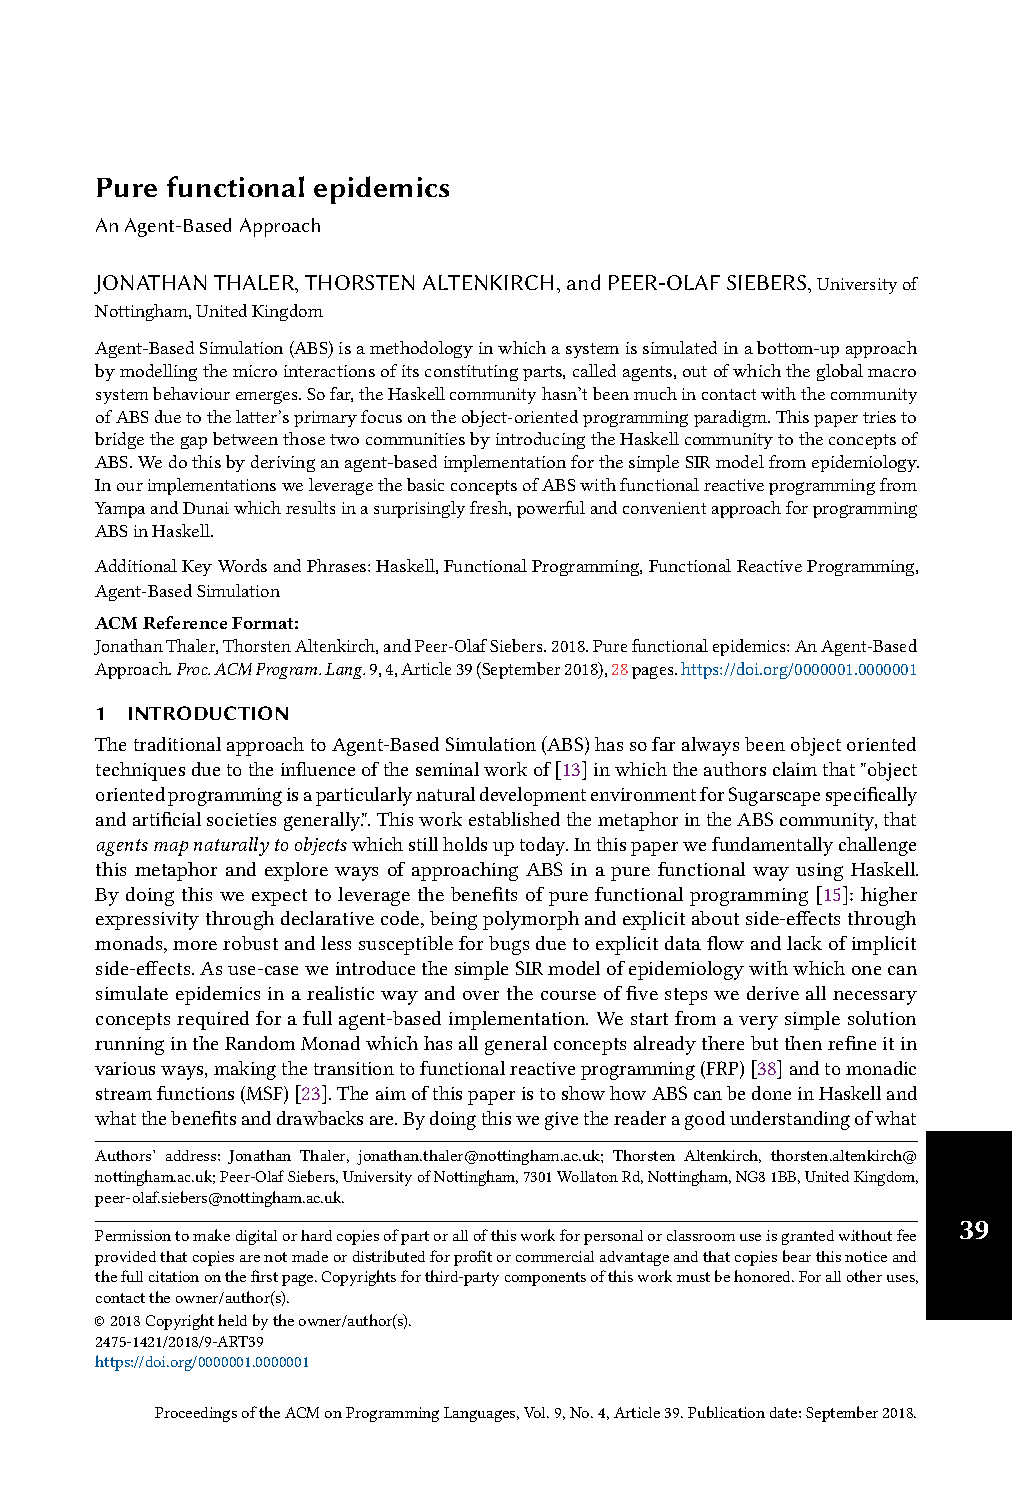
\includepdf[pages=-]{./pdf/pfe.pdf}

% NOTE: keep it out to the submission for the reviewers
%\chapter{Questions \& Answers}
\label{chap:qa}

TODO: update and adopt to 2nd year

In this chapter I give answers to anticipated questions and objections about my research direction and vision of doing pure functional ABS \footnote{They are not always posed in a dead-serious way but as it is a quite controversial topic - ABS should be done object-orientated after all huh? - I think it is appropriate. Also some objections were raised in exactly this way.}.

\paragraph{So you had this hypothesis, that pure functional programming and dependent types lead to simulation software which is more likely correct and is easier to verify and validate, right from the beginning?}
Not at all. I even had no deep knowledge of functional programming at the start of my PhD, I've just worked through the 1st edition of Grahams book "Programming in Haskell" and that's it. I had no clear understanding of purity, side-effects and Monads and I didn't know a bit about functional reactive programming. I knew that something like Dependent Types exist because Thorsten (2nd Supervisor) has sent me an email before the start of my PhD in which he pointed at Agda, so I started reading a bit about intuitionistic / constructivistic math, tried out a little bit of Agda but quickly gave up because it was way too far away (without really having mastered pure functional programming in Haskell, I believe it is nearly impossible / too difficult / makes no sense going into dependent types).
So in the beginning there was pure \textit{curiosity} about functional programming in combination with ABS because I knew nothing of FP at all and wanted to understand it (after getting bored by OO) and applying FP to ABS seemed so crazy (because everyone claims OO to be 'natural' for it) that it must be an extremely interesting challenge. I guess this is very often the case with research: there is 'just' curiosity in the beginning and then during the research process a hypothesis falls into place.


\chapter{Thesis Structure}
\label{app:thesis_struct}

TODO: find the story of my PhD thesis and connect it to my publication plan. 
TODO: story e.g. "We need functional programming to reduce the potential sources of bugs and introducing bugs harder, resulting in software which is more likely to be correct. Additionally by using dependent types we can narrow the gap between model specification and implementation even further, resulting in software which is even more likely to be correct. Further, additional benefits fall into place: purity leads to guaranteed reproducibility at compile-time, software transactional memory can be utilised to scale up to massively parallel and we have property-based testing at hand which puts the focus on specification testing rather than testing operational details".

This appendix gives a first draft of the structure outline of the thesis which I plan on start writing in April 2019. I aim for a flat structure which emphasises a strong narrative. The order of writing will be: Methodology, Proof-Of-Concept chapters, Literature Review, Discussion, Conclusions, Introduction, Abstract.
%
%line of argument
%1. established methods need extensive unit-testing for establishing correctness of software, which only increases the likelihood of correctness and doesnt guarantee it because they are inherent dynamic, testing run-time behaviour, because of the different type system.
%2. functional programming as in haskell has a strong static type system which allows to shift much much more guarantees towards static, compile-time, making many run-time tests obsolete and can guarantee a few things already at compile-time which makes tests to cover that completely obsolete
%3. dependent types can push these guarantees even further and theoretically should allow to express guarantees at compile-time to an arbitrary complex level which in theory should allow us to abandon run-time testing of bugs altogether. This does not mean that we don't need any tests anymore, as will be outlined in the chapter on Verification \& Validation \ref{chap:v_and_v}.
%4. with shifting more towards compile-time guarantees we automatically gain more confidence into the correctness of our simulation and reduce the implementation overhead of writing tests for those cases. Also some properties are simply not testable with run-time tests e.g. that some property holds forever - this is only possible to guarantee by looking at the code directly (where functional programming shines) or expressing it through compile-time guarantees. 
%5. correct by construction: narrowing the gap between model specification and implementation 
%6. Impedance Mismatch: ABS is constructive / generative in nature but the nature of the test-driven development process is deductive. is this a problem? Think of it more deeply


\section{Introduction}
This chapter is the introduction to the thesis and motivates it and describes the aim and scope of the Ph.D. Further it states the hypotheses and contributions.
\begin{itemize}
	\item Main Argument: Defining the problem, motivation, aim and scope of the Ph.D.
	\item Hypotheses: Precisely stating the hypotheses which will form the points of reference for the whole research.
	\item Contributions: Precisely list the contribution to knowledge this Ph.D. makes and list all papers which were written (and published) during this Ph.D.
\end{itemize}

\section{Literature Review}
This chapter discusses background and related work by presenting the relevant literature 

\section{Methodology}
This chapter introduces the methodology, used in the experimental chapters:

\begin{itemize}
	\item Defining and introducing Agent-Based Simulation (ABS) (History, ABS vs. MAS, examples, event- vs. time-driven).
	\item Introduce established implementation approaches to ABS (Frameworks: NetLogo, Anylogic, Libraries: RePast, DesmoJ, Programming: Java, Python, Correctness: ad-hoc, manual testing, test-driven development)
	\item Introduction Verification \& Validation (V \& V in the context of ABS).
	\item Introduction to functional Programming in Haskell (functions, types, recursion, algebraic data-types, higher-order functions, continuations, Define and explain side-effects and purity: monads, different types of effects, explain IO and that it is of fundamental importance to avoid it in our research).
	\item Introduction to dependent types (Example, Equality as Type, Philosophical Foundations: Constructive mathematics)
\end{itemize}

\section{Case Studies}
Presents case studies which are the main contribution of this Ph.D. which support our hypothesis. Each section is structured by Intro, Methods, Experiment, Analysis.

\subsection{Case Study 1: Testing and Verification}
This chapter describes how testing \& verification works in pure functional ABS.
%\begin{itemize}
%	\item Testing in functional programming
%	\item Strong Static Types rule out some classes of bugs and make some tests obsolete.
%	\item Property-Based testing: QuickCheck.
%	\item Using Property-Based testing in ABS for specification testing.
%	\item Reasoning about code
%\end{itemize}

\subsection{Case Study 2: Going Large-Scale}
This chapter discusses how pure functional ABS can go large-scale using STM. Further it is the central chapter, discussing various types of agent-agent and agent-environment interactions

%\subsubsection{Agent-Agent Interactions}
%This is the central problem of the FP approach as basically the agent-interactions define the level of abstractions over the agents. Unfortunately this is easier and more elegant in object-oriented programming. Still, by using a strong static type system we are more explicit about agent-interactions and we can have advantages which OOP doesn't have. Also we show that there are multiple different kinds of agent-interactions, depending on whether it is a time- or event-driven ABS.
%There is still much work to be done for this thesis chapter, we need to distinguish between:
%
%\begin{itemize}
%	\item Asynchronous Interaction: the flow is one-directional and does not need a listener on the other side and not a synchronous reply. The mechanism depends strongly on the type of ABS: time- or event-driven and pure or concurrent. Examples are the pure feedback in the Yampa SIR implementation, pure Data-Flow in the Yampa implementation, pure agent transactions, pure events, STM Event, STM message-boxes.
%	\item Synchronous Interactions: the flow is bi-directional and needs a listener on the other side to engage in a synchronous interaction without time-delay. We have only touched on prototyping this but need to go deeper for the final thesis. In Haskell we could build on the pure event driven approach we have implemented already in Step7\_EventDriven but we need to extend it towards an explicit synchronous mechanism. Also we need to show how we can do this in STM but there its gonna be very tricky because all agents act conceptually at the same time.
%\end{itemize}

\subsection{Case Study 3: Dependent Types}
This chapter gives an in-depth discussion on how dependent types can be made of use in pure functional ABS.

\section{Discussion}
This chapter re-visits the hypotheses and puts them into perspective of the contributions.

\section{Conclusions}
This chapter draws conclusions to the main hypothesis and outlines future research.

\section{Appendices}
Datasets, lengthy code, additional proofs.


\end{appendices}

\end{document}
